\begin{blocksection}
\question
Assume that we have a standard 5-stage pipelined CPU with no forwarding. Register file writes can happen before reads, in the same clock cycle. We also have comparator logic that begins at the beginning of the decode stage and calculates the next PC by the end of the decode stage. There is no branch delay slot (as in RISC-V). The remainder of the questions pertains to the following piece of MIPS code. Note that MIPS and RISC-V have basically identical instruction syntax but MIPS uses \$ for the registers.

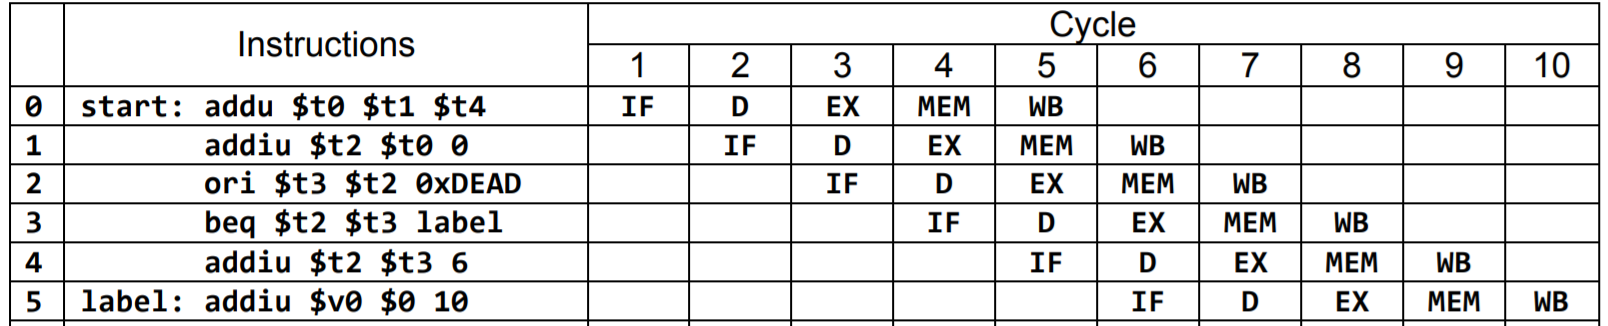
\includegraphics[width=1.4\textwidth]{images/midterm2/hazards.png}

\end{blocksection}